\chapter{Introducere}

\section{Motivație}

Conform celui mai recent raport al răspândirii metodologiei Agile\cite{annual-state-of-agile-report}, 71\% din organizațiile întrebate folosesc Agile pentru gesionarea ciclului de viață al produsului, dintre care 63\% folosesc specific Scrum. Prin contactul meu de până la momentul actual cu mediul corporate și, prin extensie, cu procesele Scrum, am observat că o piedică în maximizarea performanței unei echipe o constituie asignarea haotică a sarcinilor de lucru. Aceasta rezultă într-o lipsă de echilibru în volumul de muncă, împreună cu posibilitatea neîncheierii sarcinilor până la data limită a livrării.

Deși manifestul Agile\cite{agile-manifesto} presupune „Indivizi și interacțiune, mai presus de procese și unelte”, un studiu asupra limitărilor metodologilei\cite{agile-limitations} observă că, în practică, procesele joacă adeseori un rol important. Totuși, investiția unei perioade mari de timp în urmarea proceselor interne poate scădea considerabil din timpul rămas pentru dezvoltarea propriu-zisă, fereastra de timp alocată devenind o sursă de presiune ce poate reduce calitatea produsului final. Presiunea timpului poate împinge dezvoltatorii la a folosi soluția mai rapidă în loc de cea calitativă și minimizează importanța testării și a documentației.

Astfel, aplicația centrală acestei lucrări își propune simplificarea gestionării proiectelor din cadrul unei companii și creșterea productivității prin automatizarea procesului de atribuire a sarcinilor de lucru. Agentul de atribuire al sarcinilor de lucru face alegeri aproape instant și ar putea funcționa ca un sfătuitor imparțial, care se bazează pe analiza obiectivă și ordonată a datelor. Utilizatorii cheie sunt managerii, care pot crea panouri cu sarcini de lucru și distribui eficient volumul de muncă, și angajații obișnuiți, care își pot vizualiza sarcinile zilnice și oferi noutăți legat de statusul lor.

\section{Domenii abordate}

Această lucrare are în vedere, în principiu, domeniul dezvoltării aplicațiilor web, folosind analiza datelor pentru generarea unor sugestii potrivite. În cadrul proiectării aplicației, am folosit tehnologii mature precum Java \& Spring pentru back-end, Typescript \& React pentru front-end, PostgreSQL ca sistem de gestiune a bazelor de date relaționale, Python pentru agentul de prelucrare a datelor și Docker pentru containerizare.


\section{Nevoi îndeplinite de aplicație}

Tendințele în aria software-ului de gestiune a atribuțiilor evoluează continuu pentru a se adapta nevoilor pieței, iar cea mai semnificativă este integrarea inteligenței artificiale și a învățării automate. Aceste tehnici oferă un suport pentru predicția evoluției proiectului, prioritizarea sarcinilor și crearea unei imagini de ansamblu asupra datelor colectate. În ultimii ani, această tendință este din ce în ce mai folositoare pentru automatizarea acțiunilor repetitive și eficientizarea proceselor\cite{emerging_trends_for_effective_software}. Altă latură care necesită atenție este nevoia de instrumente care să faciliteze colaborarea în timp real. Echipe care lucrează din zone diferite ale lumii au nevoie să acceseze o platformă care oferă actualizări în timp real ale statusului proiectului, pentru o colaborare neîntreruptă. Mai mult de atât, experiența utilizatorului în aplicație trebuie să fie intuitivă, permițând utilizatorilor cu abilități tehnice variate să se adapteze ușor.

Aplicația care este subiectul tezei, „Taskage”, își propune să ofere un cadru de gestiune a sarcinilor de lucru, cu o interfață accesibilă ce oferă actualizări în timp real și un algoritm care să scadă implicarea utilizatorului în procesul de decizie și analiză a informațiilor adunate, pentru a simplifica munca managerilor, a crește echitabilitatea împărțirii volumului de muncă și a crește per total mulțumirea și productivitatea în cadrul echipei, mutând centrul atenției de la preocupări administrative la produs în sine.

Totuși, nevoile unei echipe nu coincid cu nevoile altor echipe, pe considerente precum tipul de produs, fluxul de dezvoltare al acestuia, componența și capabilitățile echipei. Chiar și metricile după care își măsoară performanță și estimările sunt diferinte de la echipă la echipă. Complexitatea atribuțiilor unui Scrum Master constă tocmai în cunoașterea tuturor aceste detalii, însă o privire de ansamblu este dificilă fără colectarea unor date și reprezentarea lor vizuală. Din aceste lucruri putem deduce că aplicația ar trebui să trateze fiecare echipă individual, pentru a se adapta la aceste nevoi greu de predefinit. Astfel, algoritmul ales analizează izolat datele colectate despre fiecare echipă, ceea ce rezolvă această problemă, dar poate fi un dezavantaj, atunci când echipa este nou formată și sugestiile nu pot fi prea informate pe baza cantității mici de date colectate.

Codul sursă al aplicației poate fi găsit la adresa \url{https://github.com/urluconceptual/taskage}.

\section{Analiza competitorilor}

Investigând cele mai populare aplicații web de gestiune a sarcinilor de lucru în cadrul unei echipe, principalele aplicații care urmăresc satisfacerea nevoilor de gestiune a proiectelor sunt:

- Jira

- Monday.com

- Azure DevOps

Fiecare dintre acestea excelează în puncte diferite și au lipsuri specifice, acoperind nevoi diferite ale procesului de gestiune a unui proiect. În continuare, am comparat aceste instrumente și am indentificat punctele forte și punctele slabe ale fiecareia.

\subsection{Jira}

Jira este un instrument de management al proiectelor dezvoltat de Atlassian și clasat pe locul 9 în domeniul dezvoltării software, cu peste 90 000 de clienți\cite{6sense-jira}. Buna lui integrare în acest context specific este relevantă din perspectiva faptului că aproape 70\% din echipele care lucrează Agile sunt echipe în domeniul IT\cite{annual-state-of-agile-report}. 

 \begin{figure}[H]
 	 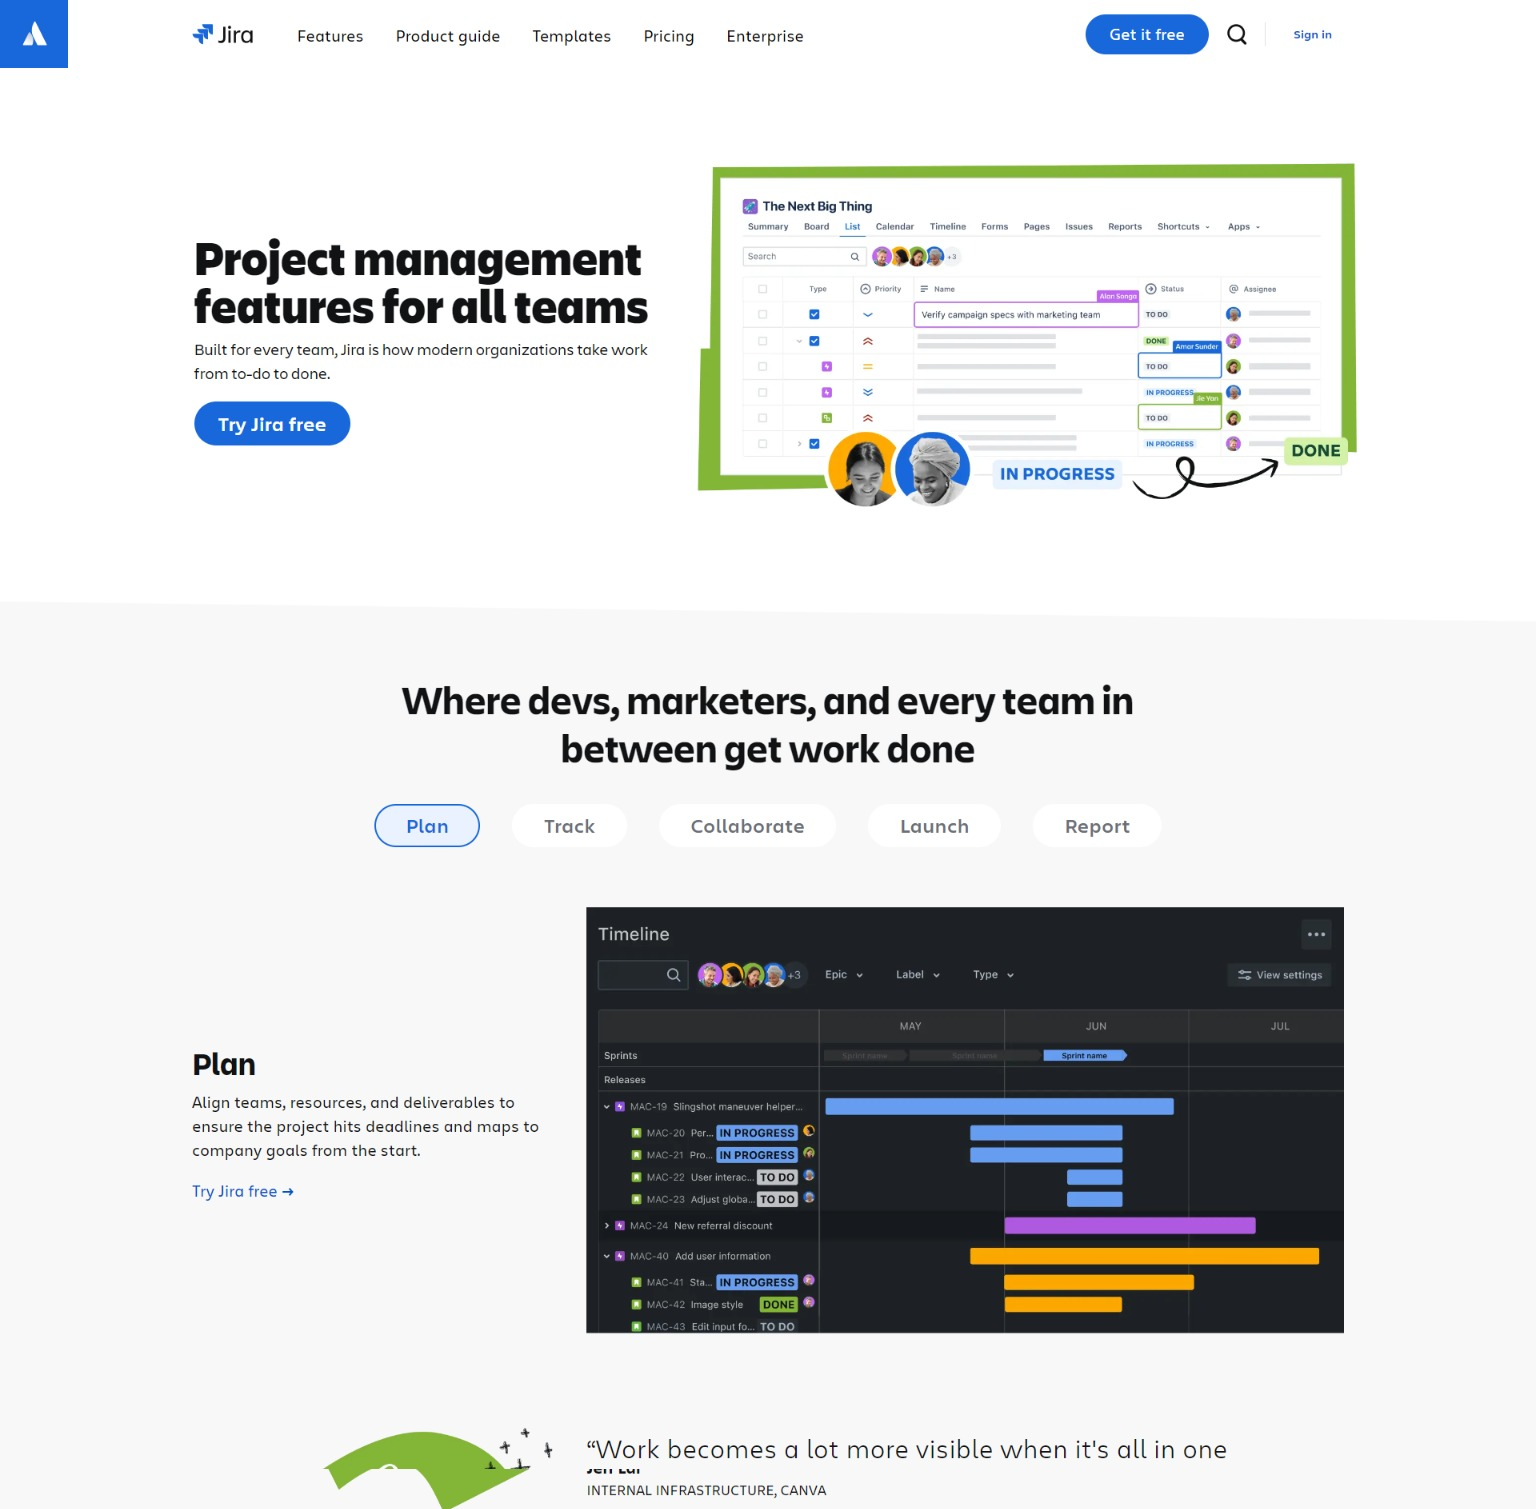
\includegraphics[width=0.5\linewidth]{jira-features-2.png}
	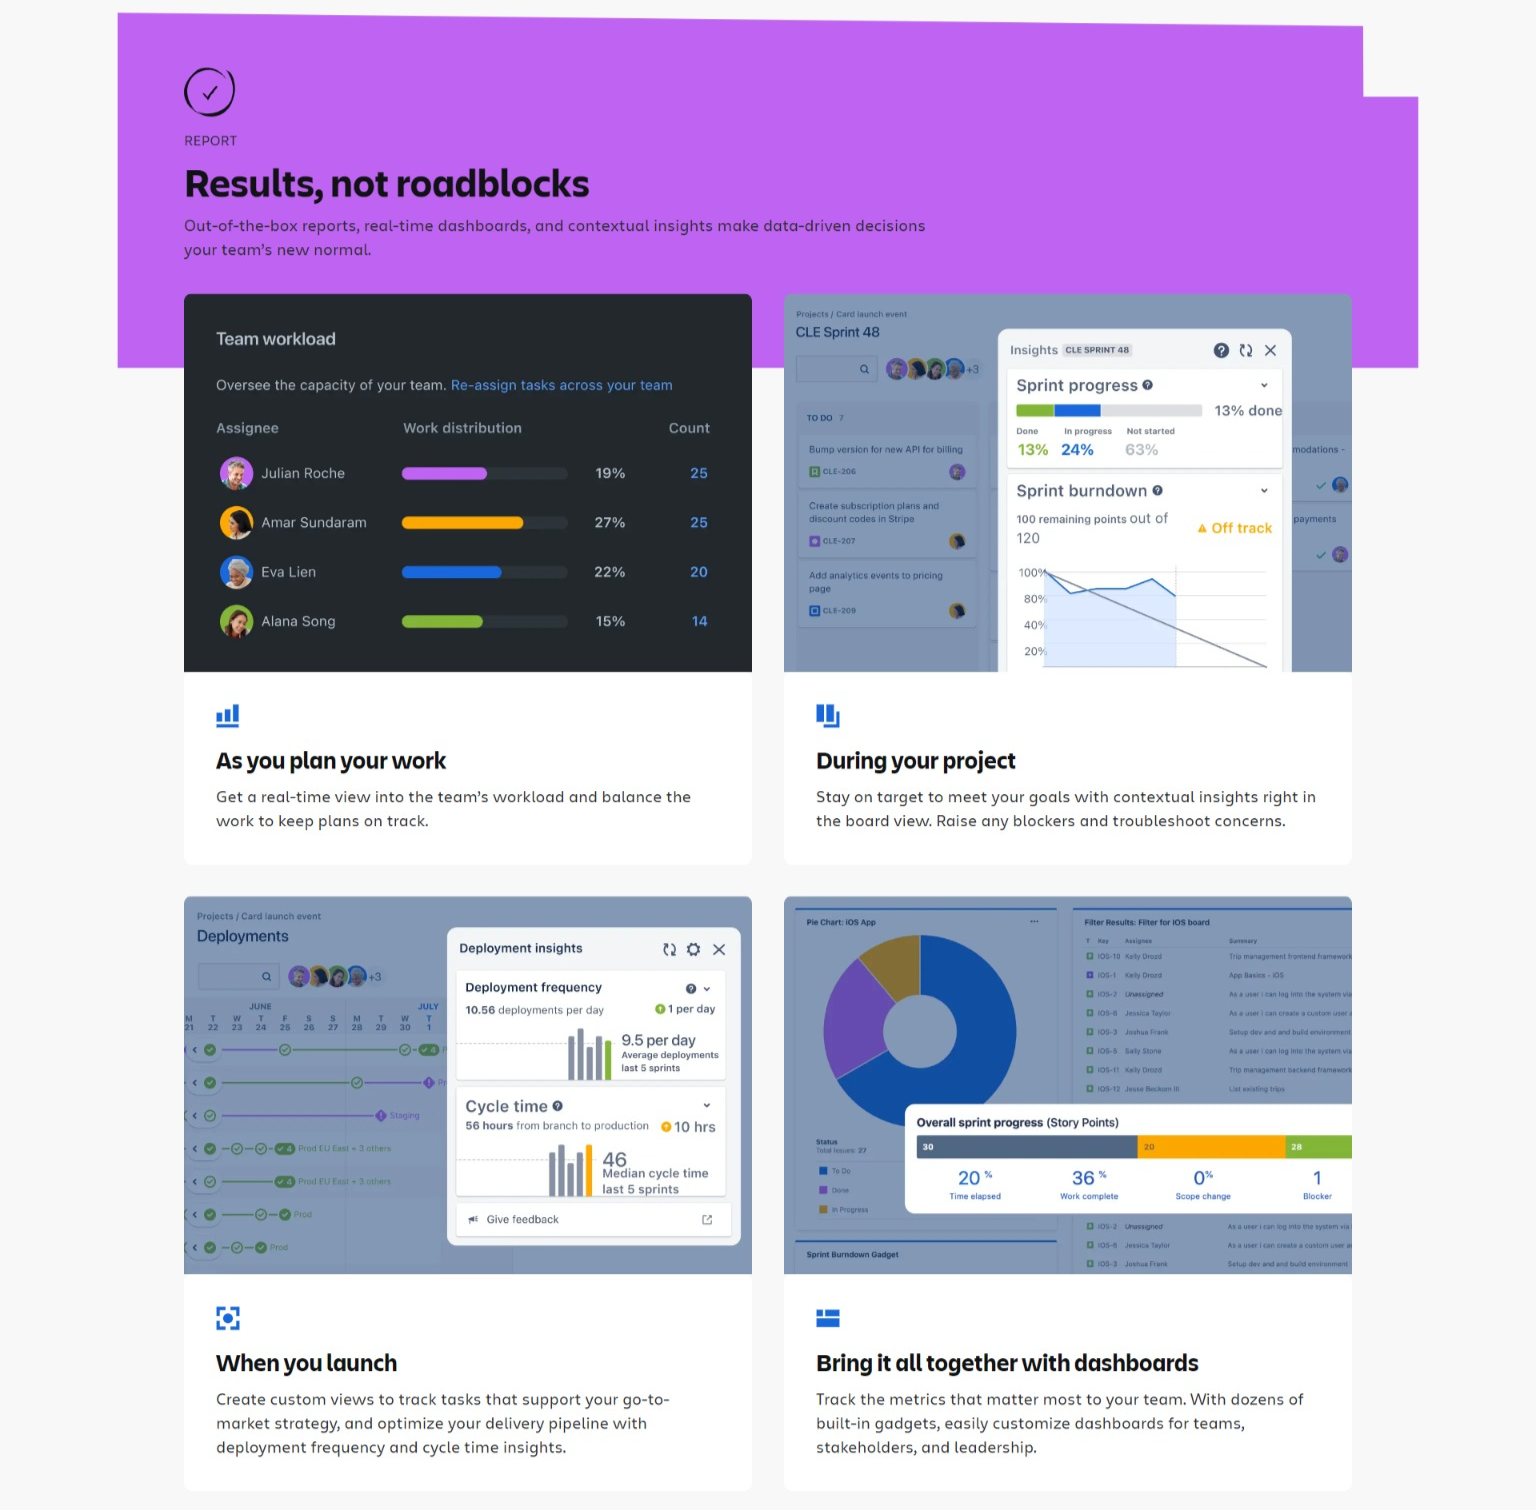
\includegraphics[width=0.5\linewidth]{jira-features-1.png}
	\caption{Jira - prezentare și funcționalități \cite{jira-features}}
	\label{fig:jira-features}
 \end{figure}

Jira oferă șabloane de gestiune pentru mai multe procese Agile, precum Scrum și Kanban. Pe lângă centralizarea datelor, acestea sunt reprezentate sub formă de rapoarte precum tabele burndown sau de analiză a velocității. De apreciat este și gradul înalt de personalizare a șabloanelor, posibilitățile de organizare a unui flux al muncii permițând echipelor să își adapteze propriul sistem. Un alt detaliu cheie este integrarea cu alte sisteme populare, precum Confluence, Bitbucket, GitHub și Slack, ce permite asocierea lui într-un ecosistem deja existent.

Deși Jira are un sistem de prețuri ce include și echipe mici, multitudinea de capabilități poate fi văzută și ca un dezavantaj din cauza timpului care trebuie investit în înțelegerea fluxurilor de utilizare. Aceasta este o piedică pentru utilizatorii noi și echipele mici, care nu au nevoie de toate aceste funcționalități. Integrarea cu numeroase alte unelte cauzează prețuri suplimentare și crește complexității gestiunii ecosistemului.

\subsection{Monday.com}

Monday.com, pe de altă parte, oferă o perspectivă mai versatilă relativ la tipurile de echipe ce îl pot folosi, cu o interfață mult mai prietenoasă utilizatorilor. Detaliul acesta este relevant urmărind raportul menționat anterior, care susține că, dintre organizațiile chestionate, 20\% implementează Agile pentru echipe non-tehnice, cum ar fi echipele de marketing și alte activități business\cite{annual-state-of-agile-report}. Prin comparație cu alte instrumente, acesta nu este clasat în topul uneltelor pentru software development, dar este clasat pe locul 16 în topul uneltelor pentru productivitate, concurând cu giganți precum Microsoft Office\cite{6sense-monday}.

 \begin{figure}[H]
	\centering
 	 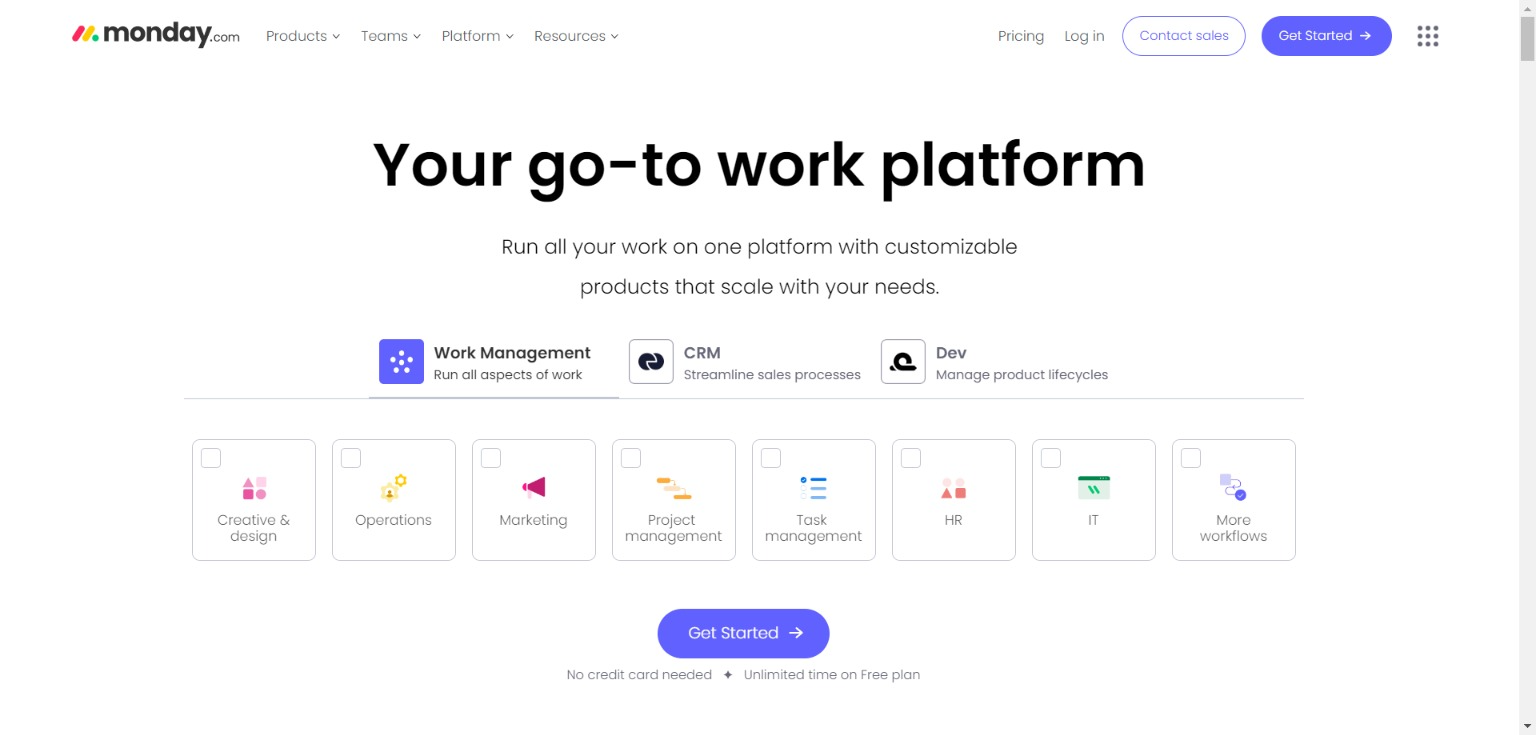
\includegraphics[width=\linewidth]{monday-features.png}
	\caption{monday.com - prezentare și funcționalități \cite{monday-website}}
	\label{fig:monday-features}
 \end{figure}

Monday.com se prezintă ca o suită de produse adaptate mai multor tipuri de echipe. Pentru echipele de dezvoltare, specifică este posibilitatea de raportare a defectelor, pentru echipele de vânzări se oferă căi de gestiune a email-urilor, iar pentru echipele de servicii clienți există opțiuni de urmărire a inventarului și a comenzilor. Experiența utlizatorului este prioritară, cu o interfață prietenoasă și reprezentări vizuale mai ușor de înțeles ale datelor \cite{monday-website}.

Ca dezavantaje, această platformă nu este potrivită echipelor de dezvoltare software prin lipsa de integrare cu unelte precum CI/CD sau versionare a codului. În plus, utilizatorii au raportat probleme de actualizare atunci când vine vorba de aplicația mobilă. Deși aștepările sunt ca o astfel de aplicație să fie folosită într-un context office, se pare că o parte din utilizatori au raportat nevoia unei variante mobile de încredere\cite{monday-cons}.

\subsection{Azure DevOps}

Azure DevOps este o alternativă de software de management pentru proiecte, dezvoltată de Microsoft. Având în vedere nevoile specifice îndeplinite de aplicație, acesta este alegerea cea mai potrivită pentru echipele de dezvoltare, fiind clasat pe locul 2 în termeni de sisteme de versionare, după GitHub\cite{6sense-azure}, chiar dacă aceasta nu este singura funcționalitate pusă la dispoziție. 

 \begin{figure}[H]
	\centering
 	 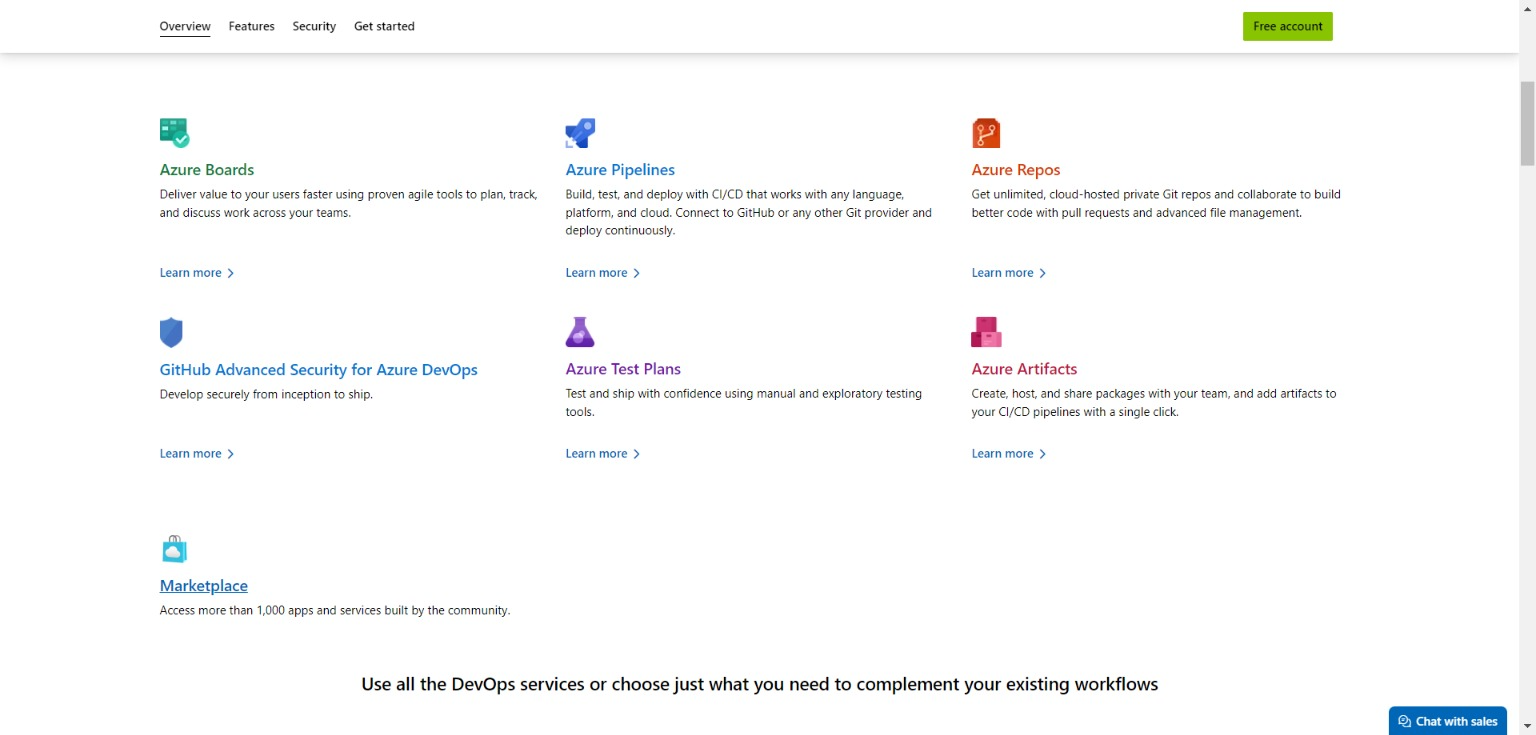
\includegraphics[width=\linewidth]{azure-features.png}
	\caption{Azure DevOps - prezentare și funcționalități \cite{azure-website}}
	\label{fig:azure-features}
 \end{figure}

Unul din avantajele principale ale aplicației Azure DevOps sunt funcționalitățile care permit gestionarea întregului ciclu de viață al unei aplicații, precum pipelines pentru CI/CD, sistem de versionare și suport pentru crearea scenariilor de testare. Faptul că toate acestea sunt asigurate de aplicație în sine face să nu fie necesară achizionarea de alte produse software. Chiar dacă este parte din ecosistemul Microsoft, aplicația oferă suport cross-platform și poate fi folosită cu tehnologii diverse. Mai mult de atât, în funcție de nevoile organizației, sunt puse la dispoziție atât opțiunea de stocare în cloud, cât și cea pe serverele companiei\cite{azure-features}. 

Asemănător cu cazul Jira, Azure DevOps necesită pregătire tehnică pentru utilizare, existând chiar și cărți și cursuri de specialitate care predau conceptele specifice. De asemenea, chiar dacă există suport cross-platform, integrarea de teste automate nu se poate face cu instrumente open-source, iar nivelul de personalizare este limitat față de ceilalți doi competitori identificați.

\subsection{Automatizare}

Atunci când vine vorba de automatizare, Jira și Monday.com pun la dispoziție un sistem bazat pe triggeri și reguli. Utilizatorul trebuie să configureze o regulă de forma „atunci când condiția … este îndeplinită, execută …”. Jira oferă varianta mai rafinată, în care utilizatorul poate descrie în limbaj natural ce dorește să automatizeze, iar sistemul va genera o serie de reguli formale pe baza mesajului. Astfel, e nevoie de efortul de analiză și decizie al utilizatorului pentru a configura toate aceste condiții. Azure DevOps, pe de alta parte, își axează posibilitățile de automatizare spre sarcinile specifice dezvoltatorilor. Spre exemplu, oferă automatizare pentru sarcinile manuale repetitive din zona de CI/CD și integrează GitHub Copilot, un instrument care sugerează blocuri de cod pe parcursul dezvoltării.

\section{Structura lucrării}

Această lucrare va prezenta implementarea și funcționalitatea aplicației „Taskage”, urmărind să explice alegerile structurale și utilizarea tehnologiilor, alese pentru a fi cât mai actuale relativ la procesele de dezvoltare întâlnite în echipe și proiecte mari. Capitolele vor acoperi ariile majore atinse de aplicație, pornind de la o perspectivă la nivel înalt și urmând prin a le detalia.
\begin{enumerate}
 	 \item \textbf{Introducere}: Prezintă contextul lucrării, incluzând motivația din spate, starea actuală a pieței și ce urmărește aplicația în sine.
	\item \textbf{Preliminarii}: Detaliză punctul de pornire al aplicației și răspunde sumar la întrebările „ce ar trebui să facă aplicația?” și „ce nevoi de implementare există?”.  Aici am identificat funcționalitățile aplicației și tehnologiile potrivite. 
	\item \textbf{Arhitectura aplicației}: Urmează cu prezentarea explicită a arhitecurii aplicației, atât ca întreg, cât și ca microservicii individuale, impreună cu diagrame suport.
	\item \textbf{Implementarea sistemului:}: Oferă detalii legat de implementarea fiecărei componente a aplicației, urmărind arii cheie precum: securitate, persistență.
	\item \textbf{Experința de utilizare și funcționalități}: Prezintă aplicația din perspectiva utilizatorului, relativ la experiența și posibilitățile acestuia de interacțiune cu aplicația.
\end{enumerate}